\chapter{Aplicación en la ciberseguridad} \label{Capitulo_3}

\section{Clasificación de Malware}

Hoy en día, uno de los principales retos que enfrenta el software anti-malware es la enorme cantidad de datos y archivos que se requieren evaluar en busca de posibles amenazas maliciosas. Una de las razones principales de este volumen tan elevado de archivos diferentes es que los creadores de malware introducen variaciones en los componentes maliciosos para evadir la detección. Esto implica que los archivos maliciosos pertenecientes a la misma ``familia'' de malware (con patrones de comportamiento similares), se modifican constantemente utilizando diversas tácticas, lo que hace que parezcan ser múltiples archivos distintos. 


Para poder analizar y clasificar eficazmente estas cantidades masivas de archivos, es necesario agruparlos e identificar sus respectivas familias. Además, estos criterios de agrupación pueden aplicarse a nuevos archivos encontrados en computadoras para detectarlos como maliciosos y asociarlos a una familia específica. 


\subsection{Microsoft Malware Classification Challenge}



El conjunto de datos utilizado en este estudio proviene del Microsoft Malware Classification Challenge (BIG 2015) \citep{kagglebig2015}, una competición dirigida a la comunidad científica. Su objetivo era promover el desarrollo de técnicas efectivas para agrupar diferentes variantes de malware en sus respectivas familias. Se puede descargar desde su página web \url{https://www.kaggle.com/c/malware-classification}, pero hay que tener en cuenta su espacio, 0.5 TB sin comprimir. Para usarla, me descargué la carpeta comprimida (7z) con todo el dataset. Después, la subí al servidor Simba de la facultad de informática y finalmente, usando el comando \textit{7zz x file\_ name.7z}, la descomprimí. 


Este dataset contiene 5 archivos:

\begin{itemize}
\item dataSample.7z - Una carpeta comprida 7z con una muestra de los datos disponibles.
\item train.7z - Una carpeta comprida 7z con los datos sin procesar para el conjunto de entrenamiento.
\item trainLabels.csv - Un archivo csv con las etiquetas asociadas a cada archivo del conjunto de entrenamiento.
\item test.7z - Una carpeta comprida 7z con los datos sin procesar para el conjunto de prueba.
\item sampleSubmission.csv - Un archivo csv que muestra el formato de envío válido de las soluciones.
\end{itemize}

Para nuestro estudio, nos enfocaremos exclusivamente en el conjunto de datos de entrenamiento, que consta de los archivos ``train.7z'' y ``trainLabels.csv''. Los archivos 'test.7z' y 'sampleSubmission.csv' están destinados específicamente para la competición. Nosotros no los utilizaremos debido a que son programas de malware sin etiquetar y para entrenar nuestras redes neuronales en este problema de clasificación de malware, es necesario conocer sus clases.  Además, la carpeta 'dataSample.7z' proporciona dos programas que se encuentran también en la carpeta train.7z, por lo que tampoco la utilizaremos en nuestro experimento. 



Cada programa malicioso tiene un identificador, un valor hash de 20 caracteres que identifica de forma única el archivo, y una etiqueta de clase, que es un número entero que representa uno de los 9 nombres de familias a los que el malware puede pertenecer \ref{tab: classMMC}. Cada programa contiene dos archivos.  Uno asm con el código extraído por la herramienta de desensamblado IDA y otro bytes con la representación hexadecimal del contenido binario del programa sin los encabezados ejecutables (para garantizar esterilidad). Para nuestro estudio vamos a utilizar únicamente este ultimo archivo. Vamos a previsualizar su estructura.

\begin{figure}[h]
    \begin{center}
    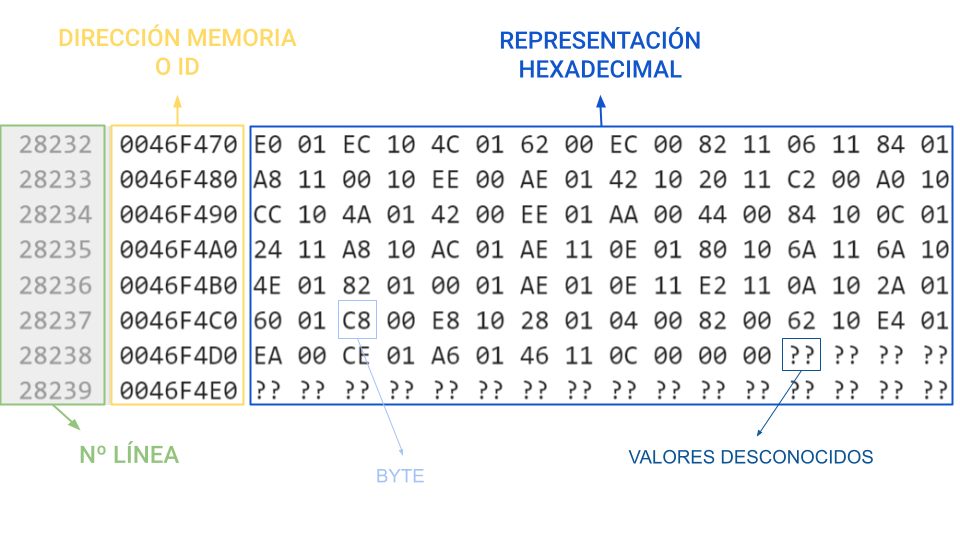
\includegraphics[width=0.8\textwidth]{img/previewMMC.png}
    \end{center}
    \caption{Previsualización del archivo``0ACDbR5M3ZhBJajygTuf.bytes'' de la carpeta train.}
    \label{fig:previewMMC}
\end{figure} 

Como aparece en \ref{fig:previewMMC}, los ocho primeros caracteres son direcciones de memoria, seguido de la representación hexadecimal del contenido binario del programa, que contiene 16 bytes (cada uno dos caracteres). A veces nos podemos encontrar con ``??'' en el lugar de un byte. Este símbolo se utiliza en estos archivos para representar que se desconoce su información porque su memoria no se puede leer \citep{cahyani2022influence}. También en \url{https://www.kaggle.com/code/dheemanthbhat/malware-classification-with-multiprocessing}.



Hay un total de 21.741 programas de malware, pero nosotros tan solo usaremos los 10868 pertenecientes al entrenamiento. Estos programas pertenecen a una de estas 9 familias de malware: Rammit, Lollipop, Kelihos\_ ver3, Vundo, Simda, Tracur, Kelihos\_ ver1, Obfuscator y Gatak. Cada una de estas familias se clasifican en una de estas 6 variadades:
\begin{enumerate}

\item Worm (Gusano)- Los gusanos informáticos son un tipo de malware que puede propagarse a través de redes sin la intervención de un programa huésped o de un humano. Son caballos de Troya maliciosos que pueden replicarse y propagarse de una computadora a otra. Los gusanos infectan a sus anfitriones mediante el engaño y la astucia, pudiendo causar graves daños a las computadoras comprometidas al consumir ancho de banda, sobrecargar sistemas, eliminar o modificar archivos e instalar virus adicionales. Además, las vulnerabilidades en el software, los archivos adjuntos de correo electrónico y las conexiones de red pueden facilitar su propagación. 

\item Adware (programa publicitario) - El adware es una variedad de malware que muestra anuncios no deseados a los usuarios, típicamente como ventanas emergentes o banners. A menudo se distribuye como parte de descargas de software gratuitas, pero también se puede obtener a través de un ciberataque o una vulnerabilidad. El adware tiene como objetivo generar ingresos para sus desarrolladores mostrando anuncios a los consumidores. Sin embargo, puede causar un daño significativo a una computadora infectada al degradar su rendimiento, reducir su disponibilidad y violar la privacidad del usuario al recopilar información sobre sus actividades de navegación.

\item Backdoor (Puerta trasera) - Un backdoor permite que una entidad no autorizada tome el control completo del sistema de una víctima sin su consentimiento. Un troyano de puerta trasera siempre se presenta como una herramienta de software legítima esencialmente requerida por el usuario. Otras opciones pueden ser visitar un sitio web malicioso o hacer clic en un enlace no deseado. Al ejecutarse, se añade a sí mismo en la rutina de inicio del sistema y busca una conexión a Internet. Una vez que el sistema está en línea, se conecta con su autor, quien luego toma el control del sistema para realizar diferentes tareas, como descargar/cargar archivos, registrar pulsaciones de teclas, enviar correos electrónicos no deseados o robar contraseñas, entre otras cosas.

\item Trojan (Troyano)- Los troyanos son programas maliciosos que se disfrazan como programas o archivos legítimos y pueden tomar el control de una computadora para ejecutar operaciones maliciosas como robar datos, dañar el sistema o abrir puertas traseras para otros virus. El término "Troyano" proviene de la leyenda griega del caballo de Troya, una táctica engañosa utilizada para conquistar Troya. En el ámbito digital, los troyanos son parásitos digitales hostiles capaces de leer contraseñas, grabar pulsaciones de teclas y propagar otros virus. Se utilizan técnicas de ingeniería social, como correos electrónicos de phishing o descargas maliciosas, para propagarlos. A diferencia de los virus informáticos y los gusanos, los troyanos no pueden replicarse y deben ser instalados o ejecutados por los usuarios.

\item Trojan downloader (Descargador troyano) - Es un programa malicioso que se descarga e instala en una computadora infectada. Puede abrir conexiones de red ilícitas, mutarse a sí mismo, deshabilitar herramientas de seguridad y transferir información personal del usuario sin permiso. Además, su función principal es la de descargar e instalar otro malware dañino en el sistema infectado.

\item Obfuscated malaware (Malware obfuscado) - La obfuscación es una técnica utilizada para hacer que el código de un programa sea más difícil de entender o de analizar. Esto implica modificar el código del programa malicioso de manera que sea más complicado para los investigadores de seguridad o los programas antivirus detectarlo y comprender cómo funciona. Su objetivo principal es eludir la detección y análisis por parte de los programas antivirus y otros sistemas de seguridad.

\end{enumerate} 

\begin{table}[htbp]
\centering
\caption{Family, Type, y Total Samples}
\begin{tabular}{ccccc}
\hline
Class ID & Familia & Tipo & Muestras & Porcentaje \\
\hline
1 & Ramnit & Worm & 1541 & 14.18 \\
2 & Lollipop & Adware & 2478 & 22.8 \\
3 & Kelihos\_ ver3 & Backdoor & 2942 & 27.07\\
4 & Vundo & Trojan & 475 & 4.37\\
5 & Simda & Backdoor & 42 & 00.39\\
6 & Tracur & Trojan Downloader & 751 & 6.91 \\
7 & Kelihos\_ ver1 & Backdoor & 398 & 3.66\\
8 & Obfuscator.ACY & Malware obfuscado & 1228 & 11.30 \\
9 & Gatak & Backdoor & 1013 & 9.32\\
\hline
\end{tabular} \label{tab: classMMC}
\end{table}


Analizando \ref{img: circularMMC}, podemos observar como la distribución entre las clases de los datos de entrenamiento no es uniforme. Mientras que de la clase Simbda 42, de la clase Kelihos\_ ver3 hay 2942, un 98 \% más. En \citep{kebede2017classification} deciden prescindir de esta clase, pero nosotros hemos decidido hacer el análisis con las 9 clases.  

\begin{figure}[h]
    \begin{center}
    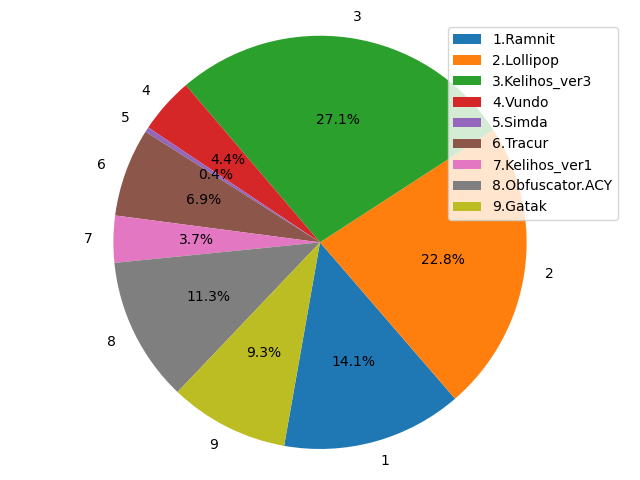
\includegraphics[width=0.8\textwidth]{img/circularMMC.png}
    \end{center}
    \caption{Distribución del BIG 2015 training dataset.}
    \label{img: circularMMC}
\end{figure}  

A la hora de crear nuestros modelos, hemos dividido el conjunto de datos aleatoriamente en grupos con el 75\%, 15\% y 10\% para entrenamiento, test y validación respectivamente. La \ref{img: train_test_valMMC} muestra como quedarían distribuidas las clases en los diferentes grupos.

\begin{figure}[h]
    \begin{center}
    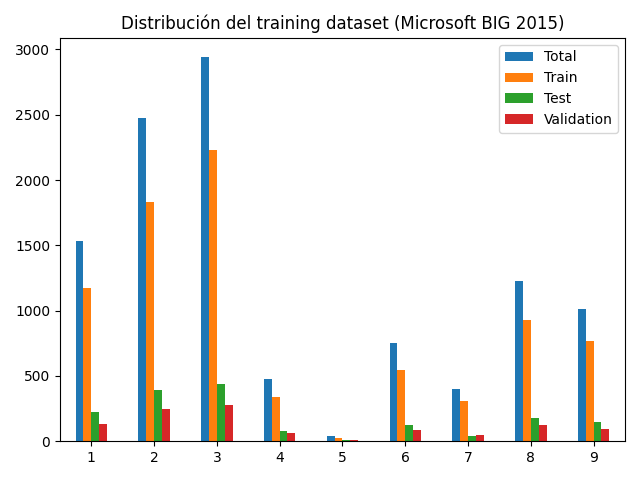
\includegraphics[width=0.8\textwidth]{img/barras4MMC.png}
    \end{center}
    \caption{Distribución de las clases en cada grupo.}
    \label{img: train_test_valMMC}
\end{figure}  


\section{Resumen del Conjunto de Datos}

El conjunto de datos utilizado en este estudio proviene del Desafío de Clasificación de Malware de Microsoft (BIG 2015), accesible a través de Kaggle. Este conjunto de datos consta de programas de malware pertenecientes a 9 categorías diferentes. Se proporcionan conjuntos de datos de entrenamiento y prueba, pero solo se utilizan los datos de entrenamiento debido a la falta de etiquetas para el conjunto de prueba para su entrega. Además

El conjunto de entrenamiento contiene 10,868 muestras de malware, cada una con un identificador único, un valor hash de 20 caracteres y una etiqueta de clase que representa una de las 9 familias de malware. Cada archivo de malware tiene una representación hexadecimal de su contenido binario, junto con un archivo 'bytes' que contiene esta información. No se excluye ninguna categoría de malware en este estudio.

La distribución de los datos se realiza con un 72\% para entrenamiento, un 8\% para validación y un 20\% para pruebas. Se realizan varias divisiones y análisis de los conjuntos de datos para ajustar y evaluar diferentes modelos y enfoques de aprendizaje profundo para la clasificación de malware.

Este conjunto de datos, con su amplia gama de muestras etiquetadas y la diversidad de familias de malware representadas, proporciona una base sólida para la investigación y desarrollo de métodos efectivos de detección y clasificación de amenazas informáticas.







Se decidió escoger este dataset y no otro porque el objetivo que tenemos en este trabajo de investigación es el de aprender y desarrollar diferentes métodos de aprendizaje automático y este dataset nos permite utilizar tanto una \acrshort{cnn} como un Autoencoder según \citep{podder2021artificial}.












\begin{comment}
un conjunto de datos de malware sin precedentes y promoviendo el desarrollo de técnicas efectivas de código abierto para agrupar variantes de archivos de malware en sus respectivas familias.

Est Fue un challenge que promocionó Microsoft para que la comunidad científica propuesiera una solución para este problema.Es un dataset que fue creado para un Challenge proporcionado por Microsoft para 
Dataset Description
Warning: this dataset is almost half a terabyte uncompressed! We have compressed the data using 7zip to achieve the smallest file size possible. Note that the rules do not allow sharing of the data outside of Kaggle, including bit torrent (why not?).

You are provided with a set of known malware files representing a mix of 9 different families. Each malware file has an Id, a 20 character hash value uniquely identifying the file, and a Class, an integer representing one of 9 family names to which the malware may belong:

Ramnit
Lollipop
Kelihos_ver3
Vundo
Simda
Tracur
Kelihos_ver1
Obfuscator.ACY
Gatak
For each file, the raw data contains the hexadecimal representation of the file's binary content, without the PE header (to ensure sterility).  You are also provided a metadata manifest, which is a log containing various metadata information extracted from the binary, such as function calls, strings, etc. This was generated using the IDA disassembler tool. Your task is to develop the best mechanism for classifying files in the test set into their respective family affiliations.

The dataset contains the following files:

train.7z - the raw data for the training set (MD5 hash = 4fedb0899fc2210a6c843889a70952ed)
trainLabels.csv - the class labels associated with the training set
test.7z - the raw data for the test set (MD5 hash = 84b6fbfb9df3c461ed2cbbfa371ffb43)
sampleSubmission.csv - a file showing the valid submission format
dataSample.csv - a sample of the dataset to preview before downloading
\end{comment}




Como podemos observar, todos los programas proporcionados son malware, lo que nos indica que con este dataset no podemos crear un modelo que nos prediga si un programa es malware o no, sino que tan solo podemos hacer un modelo de clasificación. Para ello vamos a abordar este experimento de dos formas diferentes. Una de ellas es utilizando una CNN y la otra es usando un autoencoder. utilizar dos redes neuronales
\subsection{Autoencoder}
\subsection{Red Neuronal Convolucional}
\subsection{Resultados}
El entorno de hardware en el que he realizado todos los experimentos es un sistema operativo Linux 6.1.0-17 de 64 bits con glibc2.36, funcionando en una arquitectura X86\_ 64. La CPU utilizada tiene 12 núcleos. En cuanto a la GPU, es un VGA de Intel Corporation 200 Series/Z370 Chipset Family SPI Controller con el identificador [8086:a2a4]. La memoria RAM disponible es de 126GB. 


\section{Detección de intrusiones}
\subsection{KDD Cup 1999}
\subsection{Autoencoder}
Para la clasificacion binaria usar autoencoder con el entrenamiento de las imágenes (buenas o malas) y según el error que den, se clasifica.
Para la multiclasificación, tenemos dos opciones:
\begin{itemize}
\item Usamos autoencoder para comprimir la información de entrada y despues esa informacion la usamos para clasificarla usando una DNN \citep{lopes2022effective}
\item Usamos una cadena de autoencoders en el cual la salida de h es la entrada del autoencoder h+1. Utilizo el articulo \citep{farahnakian2018deep} donde se desarrolla todo el modelo y explicacion y ademas se hace referencia al artículo \citep{bengio2006greedy} porque se basa en él (lo de salida de h es la entrada de h+1). Ver tambien:
\begin{itemize}
\item Asymmetric Stacked Autoencoder
\item Constrained Nonlinear Control Allocation based on Deep Auto-Encoder Neural Networks.

\end{itemize} El algoritmo consiste en entrenar las capas por separado en la que el input del autoencoder es la salida del autoencoder anterior. Lo que de verdad nos interesa es la capa oculta, que tiene una representación comprimida de los datos de entrada y sus pesos. Estos pesos son con los que se inicializa el entrenamiento de la stacked autoencoder acabando en softmax. He usado el url para enterlo \url{https://amiralavi.com/tied-autoencoders/}. Además en \citep{bao2017deep} explica bastante bien la diferencia entre capa autoencoder y un autoencoder.
\end{itemize}
\subsection{Red Neuronal Convolucional}
Para clasificar los datos del dataset KDD 1999 usando las \gls{cnn} vamos a seguir los siguientes articulos \citep{kim2020cnn, yang2006anomaly, nguyen2018design, kim2018encoding}. Prácticamente todo el cuerpo del experimento se encuentra en el artículo \citep{kim2020cnn}, pero en el artículo \citep{kim2018encoding} aparece la parte de normalización de los datos y algunos hiperparametros de inicio.

\subsection{Red Neuronal Profunda}
Por otro lado, el método \gls{dnn} utiliza una arquitectura muy parecida a una CNN. Podemos ver todo el procesamiento de los datos y el modelo en el artículo \citep{maithem2021network}. Además, hay buena explicacion del experimento en \citep{vigneswaran2018evaluating}. Por último, en el articulo \citep{elmasry2019empirical} están los experimentos con DNN, RNN,  RBM que puedo tomar también como referencia porque está muy bien explicado las capas e hiperparametros que utiliza.

\subsection{Red Neuronal Recurrente}
En el articulo \citep{elmasry2019empirical} están los experimentos con DNN, RNN,  RBM que puedo tomar también como referencia porque está muy bien explicado las capas e hiperparametros que utiliza.

\subsection{Restricted Boltzmann Machine}
En el articulo \citep{elmasry2019empirical} están los experimentos con DNN, RNN,  RBM que puedo tomar también como referencia porque está muy bien explicado las capas e hiperparametros que utiliza.


\subsection{Resultados}
El entorno de hardware en el que he realizado todos los experimentos es un sistema operativo Linux 6.1.0-17 de 64 bits con glibc2.36, funcionando en una arquitectura X86\_ 64. La CPU utilizada tiene 12 núcleos. En cuanto a la GPU, es un VGA de Intel Corporation 200 Series/Z370 Chipset Family SPI Controller con el identificador [8086:a2a4]. La memoria RAM disponible es de 126GB.



